\documentclass[12pt,english]{article}
\usepackage{geometry}
\usepackage{float}
\usepackage{caption}
\geometry{verbose,tmargin=3cm,bmargin=3cm,lmargin=3cm,rmargin=3cm}
\usepackage{amsmath}
\usepackage{amssymb}
\usepackage{amsthm}
\usepackage{adjustbox}
\usepackage{hyperref}
\usepackage{graphicx}
\usepackage{setspace}
\onehalfspacing
\usepackage{babel}
\newcommand{\expec}{\ensuremath{\mathbb E}}
\begin{document}
\begin{center}
{\Large{}Section 1: Introduction, Solow Model\footnote{These section notes are based off notes created by Zhimin Li.}}
\par\end{center}{\Large \par}

\begin{center}
EEP 152
\par\end{center}

\begin{center}
August 31, 2016
\par\end{center}

\begin{itemize}
	\setlength\itemsep{-0.5em}
	\item Introduction (10 min)
	\item Solow model (math) (20 min)
	\item Solow model (motivating the course) (20 min)
\end{itemize}

\section{Introduction}

See section syllabus.

\section{Solow model (math)}

\subsection{Setup}

As we saw the first day of class, per capita income is strongly predictive of welfare, so understanding why some countries have higher incomes and some countries have lower incomes will take us a long way to understand variation in welfare. The Solow model presents one explanation for the source of this variation - differences in the ``capital stock'' (think industrialization, buildings, machines, \ldots).

We assume each country's income is a function of two things - its effective population (number of workers, adjusted for human capital), and its capital stock. We further assume
\begin{itemize}
	\item Income is constant returns to scale in effective population and capital stock (if we double effective population and capital stock, income doubles)
	\item Marginal product of capital and effective workers is positive (adding another unit of capital increases income, adding another unit of effective workers increases income)
	\item Decreasing marginal product of capital (the $(i+1)$th unit of capital you add increases production by less than the $i$th unit of capital, all else equal)
\end{itemize}

One convenient function that satisfies these assumptions is
$$ \underbrace{Y_{t}}_{\substack{\text{income,} \\ \text{period } t}} = ( \underbrace{K_{t}}_{\substack{\text{capital stock,} \\ \text{period } t}} )^{\alpha} ( \underbrace{E_{t}}_{\substack{\text{labor augmenting} \\ \text{technology, period } t}} \underbrace{P_{t}}_{\substack{\text{population,} \\ \text{period } t}} )^{1 - \alpha} $$

$E_{t} P_{t}$ is the units of effective workers - doubling $E_{t}$ (how productive workers are) or doubling $P_{t}$ (number of workers) has the same effect on income $Y_{t}$. We next assume
\begin{itemize}
	\item A share $s$ of income goes to investment, which increases the capital stock next period ($K_{t + 1}$)
	\item A share $\delta$ of the capital stock is lost each period
\end{itemize}
Together, these imply
$$ \underbrace{K_{t + 1}}_{\substack{\text{capital stock,} \\ \text{period } t + 1}} = \underbrace{(1 - \delta) K_{t}}_{\substack{\text{depreciated period } t \\ \text{capital stock}}} + \underbrace{s Y_{t}}_{\text{investment}} $$
We can simplify both of these expressions by dividing through by the number of effective workers, $E_{t} P_{t}$, to understand the evolution of capital per effective worker (which we can call ``capitalization''), which in this model determines the evolution of income per effective worker. This yields
\begin{align*}
\text{Income: } & \widehat{y_{t}} = \left( \widehat{k_{t}} \right)^{\alpha} \\
\text{Law of motion: } & (1 + \pi) (1 + n) \widehat{k_{t+1}} = (1 - \delta) \widehat{k_{t}} + s \widehat{y_{t}}
\end{align*}
where $\pi$ is the growth rate of technology $\frac{E_{t+1} - E_{t}}{E_{t}}$, and $n$ is the growth rate of population $\frac{P_{t + 1} - P_{t}}{P_{t}}$. In the income equation, we can see income per effective worker only depends on capitalization (capital per effective worker), so understanding the evolution of capitalization is sufficient to understand the evolution of income per effective worker. So the law of motion for capital is where we'll focus our analysis.

\subsection{Dynamics and a steady state}

How does capital evolve? We can rewrite the law of motion as
$$ \widehat{k_{t+1}} = \frac{1 - \delta}{(1 + \pi)(1 + n)} \widehat{k_{t}} + \frac{s}{(1 + \pi)(1 + n)} \widehat{y_{t}} $$
Lets plot this evolution for three cases : a country beginning with a very low, low, and high level of initial capitalization. We assume all three countries have the same values of $\delta$, $\pi$, $n$, and $s$. We'll put $\widehat{k_{t + 1}}$ on the vertical axis and $\widehat{k_{t}}$ on the horizontal axis. We'll also plot the 45 degree line, so once we calculate $\widehat{k_{t + 1}}$, we can use that to go back to the horizontal axis and calculate $\widehat{k_{t + 2}}$.

\newpage
\begin{center}
\begin{adjustbox}{
		max width=0.65\textwidth,
	}
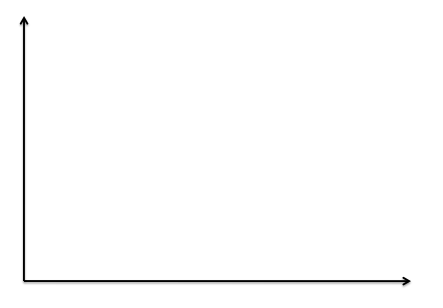
\includegraphics{axes.png}
\end{adjustbox}
\begin{adjustbox}{
		max width=0.65\textwidth,
	}
	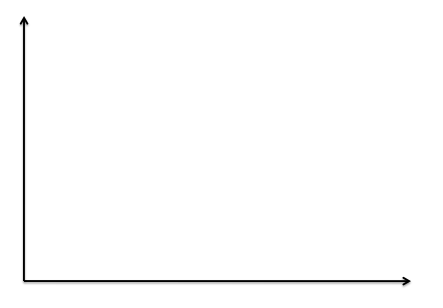
\includegraphics{axes.png}
\end{adjustbox}
\begin{adjustbox}{
		max width=0.65\textwidth,
	}
	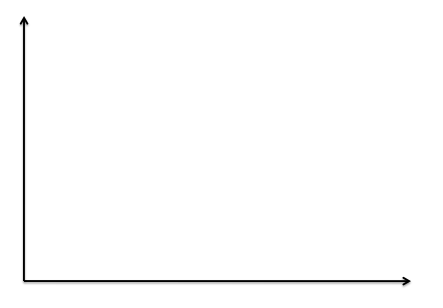
\includegraphics{axes.png}
\end{adjustbox}
\end{center}

You should note two main things:
\begin{itemize}
	\item All three countries converge to the same steady state, where $\widehat{k_{t + 1}} = \widehat{k_{t}}$, with identical capitalization $\widehat{k^{*}}$
	\item Countries further from the steady state converge faster
\end{itemize}

Finally, given $\delta$, $n$, $\pi$, $s$, and $Y_{t}(K_{t}, E_{t} L_{t})$ (income as a function of capital and effective workers), we'll often use the model to answer two questions.
\begin{itemize}
	\item How does the capital stock $K_{t}$ evolve?
	\begin{itemize}
		\item Plug in parameters and starting values of the capital stock $K_{t}$ and effective worker stock $E_{t} L_{t}$ into the law of motion.
	\end{itemize}
	\item What is the steady state level of capitalization $\widehat{k^{*}}$?
	\begin{itemize}
		\item Solve $\widehat{k_{t + 1}} = \widehat{k_{t}}$. To do this, substitute the law of motion for $\widehat{k_{t + 1}}$, which gives $\widehat{k_{t + 1}}$ as a function of $\widehat{k_{t}}$, then solve for $\widehat{k_{t}}$.
	\end{itemize}
\end{itemize}

\section{Solow model (motivating the course)}

We've seen that the Solow model predicts that countries with the same values of the growth parameters ($n$, $\delta$, $\pi$, $s$) should experience convergence in income per effective worker. As mentioned in class, there are persistent gaps in income per capita across countries, and although variation in $n$ and $s$ may exist, it does not explain the magnitude of variation in income per capita across countries. Technology and depreciation should also be identical across countries.\footnote{For now, let's think about education, which could in our model drive big differences in $E_{t}$ across countries, as human capital that countries can invest it. The puzzle remains similar - investment in human capital should have higher returns in countries with low initial human capital stocks, once again generating convergence.}\footnote{Geographic differences (such as climate, access to ports) might plausibly lead to differences in levels of productivity, but they don't explain anything close to the degree of variation in both levels and growth rates of per capita income that we observe.}

Since it seems then that poor and rich countries should move to a steady state, but incomes are not converging, we'll then consider the possibility that there are multiple steady states - in other words, that poor countries are stuck in poverty traps.

\subsection{Poverty traps}

\begin{center}
	\begin{adjustbox}{
			max width=0.8\textwidth,
		}
		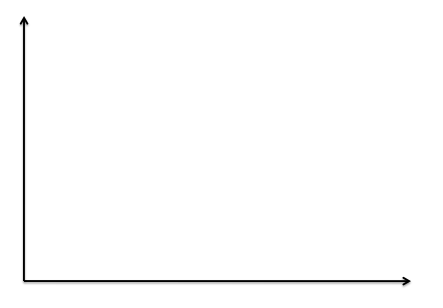
\includegraphics{axes.png}
	\end{adjustbox}
\end{center}
A poverty trap is generated when, at moderate, but not low, levels of income, increases in income lead to much larger increases in capitalization. We discussed one possibility - that $s$ is increasing in income. Another possibility is that the ``magic'' by which $sY_{t}$ becomes $K_{t+1}$ is not so magical - many different types of investments are possible, some increase income by more than others, and the better investments are not possible to make (for some reason) in low income countries. What types of poverty traps might exist? How could we test for the existence of those poverty traps?
\begin{itemize}
	\item 
	\item
	\item
	\item
	\item
	\item
	\item
\end{itemize}

\end{document}